\section{Introduction}
\label{sec:introduction}

% P:I1
Graph intervention asks which change to a network best improves a global objective, as in link optimization for opinion dynamics or information access~\cite{zhu2021polarization,liu2026accessfairness}. When edits are applied in sequence, each choice changes the problem faced by the next. We study this task under the signed Friedkin--Johnsen model, where fixed input opinions and positive or negative interactions determine the expressed equilibrium~\cite{friedkin1990opinions,zhou2024signedfj}. The objective is equilibrium energy: the squared magnitude of expressed opinions plus weighted signed disagreement. An edit's \emph{gain} is its reduction in this energy. A request asks the service to choose improving edits from a legal catalog, with a specified tolerance and tie order. Certifying such a choice requires evidence about both its gain and its competitors.

% P:I2
The difficulty is that a local edit can change the equilibrium throughout the network. A candidate rejected earlier may become attractive even though its own edge is untouched. On a three-vertex path with two negative edges and only their negative-to-positive flips permitted, the right flip initially increases energy. After the left flip, the right flip decreases energy and becomes the best remaining choice (Proposition~\ref{prop:revival}). The second decision needs evidence valid for the updated state.

% P:I3
This creates a data management problem at the intersection of selective ranked access~\cite{bruno2002webtopk,guo2008querydependent} and incremental analytics~\cite{Koch_2014,Nikolic2014Linview}. Evaluating one contender may require a global linear solve, even though only a few endpoint quantities enter its gain. Meanwhile, allowing every missing edge to be inserted gives a sparse graph a quadratic candidate space. An explicit index materializes that space; streaming avoids the table but repeatedly scans it. Response reuse targets the numerical cost, while bounds on unexamined candidates target the access cost.

% P:I4
J-CERT+ separates the numerical information used to score an edit from the coverage bounds used to choose it (Figure~\ref{fig:system}). The response layer selectively maintains small endpoint summaries and transfers them across edits with certified error bounds. The coverage layer accounts for every legal alternative using bounds valid for the current graph and request. These bounds direct response acquisition toward contenders; the resulting gain intervals in turn sharpen the decision threshold. The service can therefore reuse numerical work while establishing a complete basis for each new choice.

% P:I5
We instantiate this design for positive insertions at a common weight on all initially missing edges and magnitude-preserving flips of initially negative edges. H covers this mixed catalog through ordered insertion rows and an ordered flip list. G first tests whether a flip can exclude all insertions, then uses disjoint insertion blocks when needed. Each path provides complete coverage through its own access structure. Both share the response layer with explicit indexing (D) and bounded streaming (S).

% P:I6
Finite precision connects the access and response layers. J-CERT+ propagates errors in maintained summaries and encloses computed gains in conservative intervals. It compares a proposed winner's lower bound with upper bounds on all rivals, using checked structural equalities to resolve supported ties. Every accepted edit satisfies the same positivity, coverage, and tie requirements, whichever access path supplies the candidates.

% P:I7
Experiments on Bitcoin Alpha and OTC show how the two layers affect complete service cost. In the instrumented D/S/H comparison, H reduces aggregate setup-plus-service time by a factor of 3.79 relative to D across 15 matched repetitions on five completed confirmation streams. A separate common-lightweight comparison on the same inputs gives G 12.56\% lower aggregate cost than H: cheaper coverage preparation offsets greater response demand. Independent full-catalog replay verifies all 30 decisions in two preselected H requests.

\begin{figure*}[t]
\centering
% Preserve the supplied PNG. The two inter-layer labels are corrected in the
% typesetting layer: contenders flow down; certified gain bounds flow up.
\begin{tikzpicture}
\node[anchor=south west,inner sep=0] (figone) at (0,0)
  {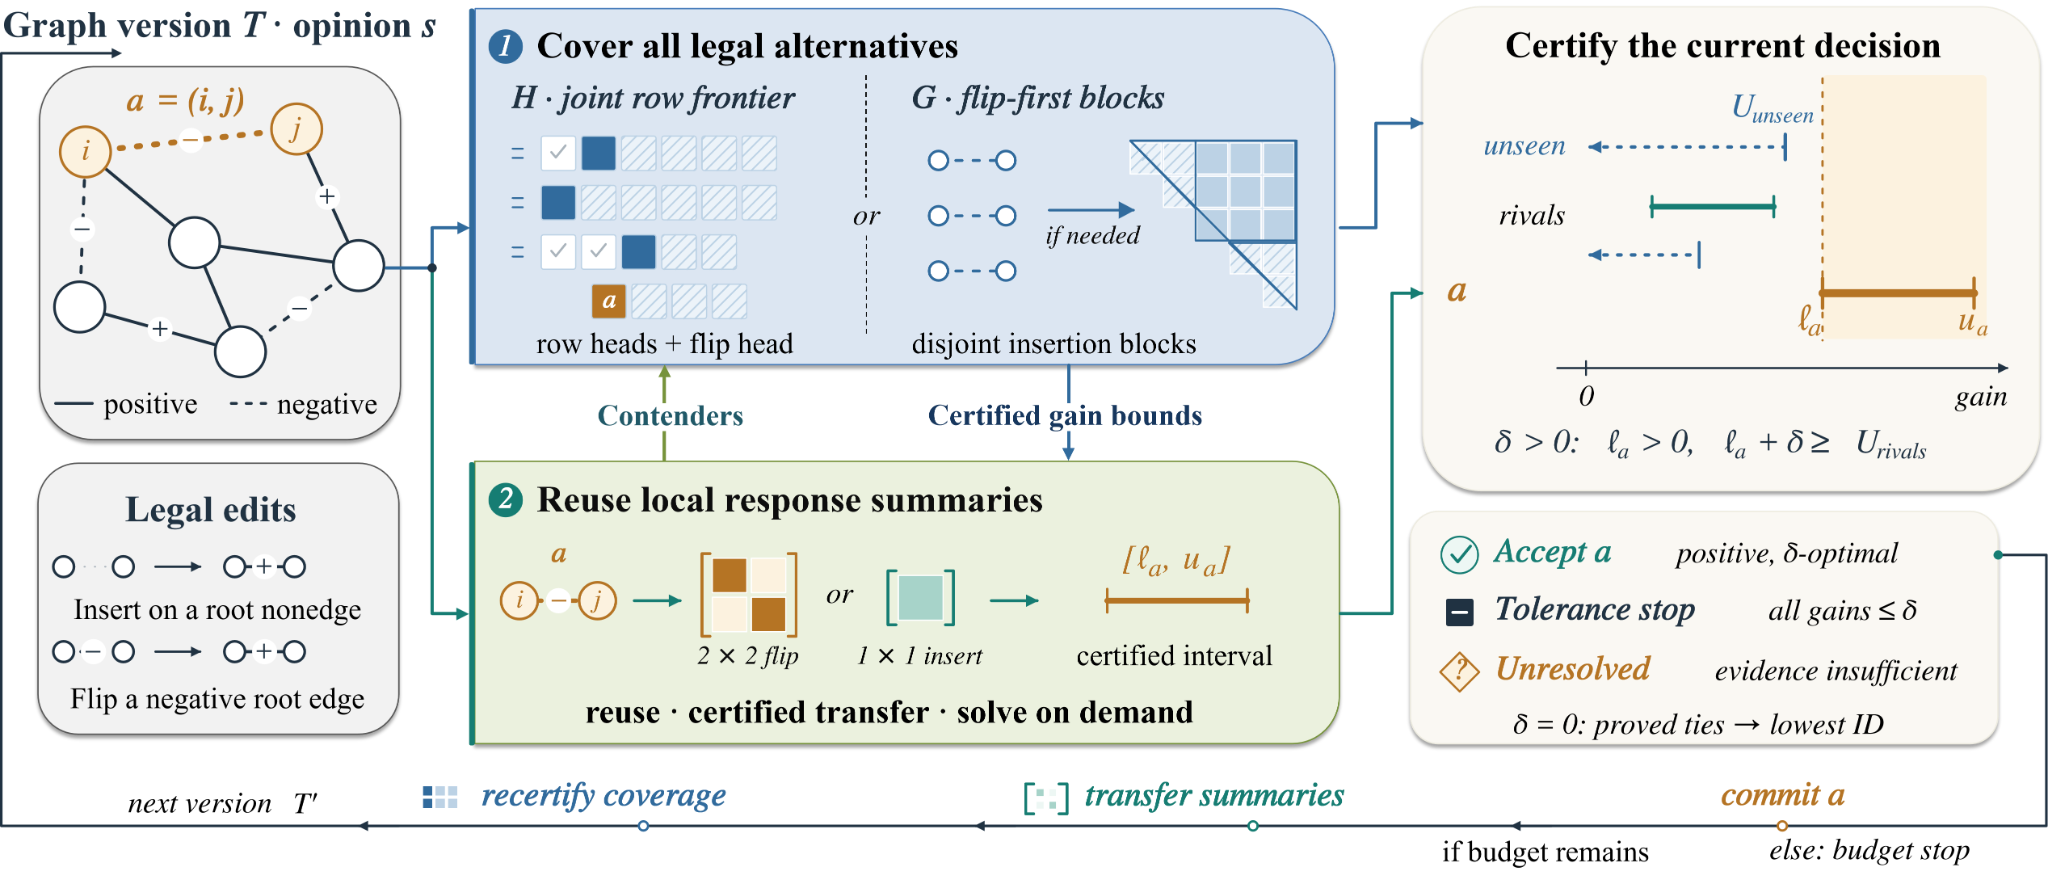
\includegraphics[width=\textwidth]{user_originals/fig1.png}};
\begin{scope}[x={(figone.south east)},y={(figone.north west)}]
\fill[white] (0.2441,0.4994) rectangle (0.6006,0.5420);
\node[font=\bfseries\fontsize{7.2}{8}\selectfont,text=teal!65!black,inner sep=0]
  at (0.3242,0.5207) {Certified gain bounds};
\node[font=\bfseries\fontsize{7.2}{8}\selectfont,text=blue!45!black,inner sep=0]
  at (0.5215,0.5207) {Contenders};
\end{scope}
\end{tikzpicture}
\caption{Current coverage and reusable responses cooperate to certify each edit. H's row frontier or G's block cover identifies contenders; local responses return certified gain bounds. At graph version $T$ with opinion $s$, $[\ell_a,u_a]$ encloses candidate $a$'s gain, $U_{\mathrm{rivals}}$ bounds every other legal candidate, including unseen ones, and $\delta$ is the selection tolerance. An accepted edit advances the version, transfers summaries, and re-establishes coverage while budget remains.}
\Description{A signed graph and its legal edits feed two cooperating layers. Coverage sends contenders to the response layer, which returns certified gain bounds. The current decision combines bounds on unseen candidates and evaluated rivals with a candidate's gain interval. An accepted edit transfers summaries and establishes coverage for the next graph version.}
\label{fig:system}
\end{figure*}

